\begin{tikzpicture}
	
	\onslide<1->{
		
		\node[inner sep=0pt] (A) at (3,0)
		{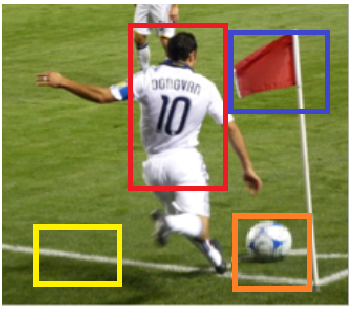
\includegraphics[scale = 0.45]{images/input.png}};
		\draw[black, thick, ->]  (4.5,0) --  (5,0);
	}

	\onslide<2->{
		\node [text width = 30mm] at (6,3){Region proposals};
		\node[inner sep=0pt] (A) at (6,0)
		{
\includegraphics[scale = 0.55]{images/region_proposals.png}};

		\draw[black, thick, ->]  (7,-0.85) --  (7.7,-0.85);
		\draw[black, thick, ->]  (7,-2.15) --  (7.7,-2.15);
		\draw[black, thick, ->]  (7,0.35) --  (7.7,0.35);
		\draw[black, thick, ->]  (7,1.85) --  (7.7,1.85);
	}

	\onslide<4->{
		\tikzstyle{input_neuron}=[circle,draw=red!50,fill=red!10,thick,minimum size=6mm]
		\tikzstyle{hidden_neuron}=[circle,draw=blue!50,fill=cyan!10,thick,minimum size=6mm]
		\tikzstyle{output_neuron}=[circle,draw=green!50,fill=green!10,thick,minimum size=6mm]
		\tikzstyle{cpy_neuron}=[circle,draw=red!50,fill=red!50,thick,minimum size=6mm]
		\tikzstyle{input}=[circle,draw=black!50,fill=black!20,thick,minimum size=6mm]
		\node [text width = 34mm] at (10,3){Feature extraction};
		\node [input_neuron] (neuron51) at (8.5,1.85) {} ;
		\node [input_neuron] (neuron52) at (9.5,1.85)  {};
		\node [input_neuron] (neuron53) at (10.5,1.85)  {};
		\node [input_neuron] (neuron54) at (11.5,1.85)  {};
		\node [text width = 5mm] at (8.7,1.1){$x_1$};
		\node [text width = 5mm] at (9.7,1.1){$x_2$};
		\node [text width = 5mm] at (10.7,1.1){$\dots$};
		\node [text width = 5mm] at (11.7,1.1){$x_d$};
		\draw[red!100,thick,solid,rounded corners=15pt] (8,2.35) rectangle (12,1.35);
	}
	
	\onslide<5->{
		\node [text width = 25mm] at (14.5,3){\ \ \ Classifier};
		\node [text width = 10mm] at (12.8,2.6){person};
		\node [text width = 10mm] at (14,2.6){flag};
		\node [text width = 10mm] at (15,2.6){ball};
		\node [text width = 10mm] at (16,2.6){none};
		\draw[black, thick, ->] (12.1,1.85) --  (12.4,1.85);
		\node [output_neuron] (neuron51) at (13,1.85) {} ;
		\node [output_neuron] (neuron52) at (14,1.85)  {};
		\node [output_neuron] (neuron53) at (15,1.85)  {};
		\node [output_neuron] (neuron54) at (16,1.85)  {};
		\draw[red!100,thick,solid] (12.5,2.35) rectangle (16.5,1.35);
		\node [cpy_neuron] (neuron01) at (13,1.85) {};
	}

	\onslide<4->{
		\node [input_neuron] (neuron51) at (8.5,0.35) {} ;
		\node [input_neuron] (neuron52) at (9.5,0.35)  {};
		\node [input_neuron] (neuron53) at (10.5,0.35)  {};
		\node [input_neuron] (neuron54) at (11.5,0.35)  {};
		
		\draw[red!100,thick,solid,rounded corners=15pt] (8,0.85) rectangle (12,-0.15);
	} 
	
	\onslide<5->{
		
		\draw[black, thick, ->] (12.1,0.35) --  (12.4,0.35);

		\node [output_neuron] (neuron51) at (13,0.35) {} ;
		\node [output_neuron] (neuron52) at (14,0.35)  {};
		\node [output_neuron] (neuron53) at (15,0.35)  {};
		\node [output_neuron] (neuron54) at (16,0.35)  {};
		
		\draw[red!100,thick,solid] (12.5,-0.15) rectangle (16.5,0.85);
		
		\node [cpy_neuron] (neuron01) at (14,0.35) {};
	}
	
	
	\onslide<4->{
		
		\node [input_neuron] (neuron51) at (8.5,-0.85) {} ;
		\node [input_neuron] (neuron52) at (9.5,-0.85)  {};
		\node [input_neuron] (neuron53) at (10.5,-0.85)  {};
		\node [input_neuron] (neuron54) at (11.5,-0.85)  {};
		
		\draw[red!100,thick,solid,rounded corners=15pt] (8,-1.35) rectangle (12,-0.35);
	} 
	
	
	\onslide<5->{
		
		\draw[black, thick, ->] (12.1,-0.85) --  (12.4,-0.85);

		\node [output_neuron] (neuron51) at (13,-0.85) {} ;
		\node [output_neuron] (neuron52) at (14,-0.85)  {};
		\node [output_neuron] (neuron53) at (15,-0.85)  {};
		\node [output_neuron] (neuron54) at (16,-0.85)  {};
		
		\draw[red!100,thick,solid] (12.5,-1.35) rectangle (16.5,-0.35);
		
		\node [cpy_neuron] (neuron01) at (15,-0.85) {};
	}
	
	\onslide<4->{
		\node [input_neuron] (neuron51) at (8.5,-2.15) {} ;
		\node [input_neuron] (neuron52) at (9.5,-2.15)  {};
		\node [input_neuron] (neuron53) at (10.5,-2.15)  {};
		\node [input_neuron] (neuron54) at (11.5,-2.15)  {};
		
		\draw[red!100,thick,solid,rounded corners=15pt] (8,-2.65) rectangle (12,-1.65);
	} 
	
	
	\onslide<5->{
		
		\draw[black, thick, ->] (12.1,-2.15) --  (12.4,-2.15);
		\node [output_neuron] (neuron51) at (13,-2.15) {} ;
		\node [output_neuron] (neuron52) at (14,-2.15)  {};
		\node [output_neuron] (neuron53) at (15,-2.15)  {};
		\node [output_neuron] (neuron54) at (16,-2.15)  {};
		
		\draw[red!100,thick,solid] (12.5,-2.65) rectangle (16.5,-1.65);
		
		\node [cpy_neuron] (neuron01) at (16,-2.15) {};
	}
\end{tikzpicture}